\chaptertitle{第十章\quad 极端原理与组合最值}

极端原理是组合数学中一种非常"聪明"的方法——当问题涉及一大堆对象时，考虑其中"最大"、"最小"、"最极端"的那一个，往往能让你找到突破口。本章先学习极端原理，再学组合最值问题的构造与证明。

\sectiontitle{10.1\quad 极端原理}

极端原理的基本思路是：从最特殊、最极端的情况出发，利用它的极端性质来推出一般结论。

几个常用角度：
\begin{itemize}
\item 取最大（最长、最高、最重）的那一个。
\item 取最小（最短、最低、最轻）的那一个。
\item 取边界上的那一个。
\end{itemize}

\begin{example}
证明：任意$n$个人中，必有两个人握手的次数相同。
\end{example}
\begin{solution}
每个人最多握$n-1$次手（除了自己）。握手次数有$0,1,2,\dots,n-1$共$n$种可能。\\
如果一个人握了$n-1$次（跟所有人握了），则没有人握$0$次。\\
如果一个人握了$0$次（跟没人握），则没有人握$n-1$次。\\
所以实际上可能的握手次数只有$n-1$种（去掉$0$和$n-1$中的一个）。\\
$n$个人分配到$n-1$种次数，必有两人次数相同。
\end{solution}

\begin{example}
平面上有$n$个点，任意三点不共线。证明：存在三个点构成的三角形，以这三个点为顶点，其内部（含边上）不包含任何其他给定点。
\end{example}
\begin{solution}
考虑所有以给定点为顶点的三角形中，面积最小的那个。
这个三角形内部不可能有任何其他给定点——如果有，那个点与其他两个顶点构成的三角形面积会小于这个最小面积，矛盾。
\end{solution}

\begin{example}
黑板上写着$1,2,3,\dots,100$。每次操作可以擦去任意两个数$a,b$，并写上$\dfrac{a+b}{2}$。经过多次操作后，最后剩下一个数。这个数最小可能是多少？最大可能呢？
\end{example}
\begin{solution}
先观察不变量。每次操作后，所有数的和的变化：$a+b$变成$\dfrac{a+b}{2}$，总和减少$\dfrac{a+b}{2}$。\\
所以不变量不是总和。换一个思路：最大值和最小值的变化。\\
每次操作选两个数取平均，新数一定介于原来的两数之间。\\
所以最大值只能减小（当选到最大数时），最小值只能增大（当选到最小数时）。\\
最终剩下的数一定是$\ge$原来的最小值（$1$）且$\le$原来的最大值（$100$）。\\
具体能到什么值，取决于操作顺序——它可以是$1$到$100$之间的任何数以$\dfrac12$为步长的值？实际上不完全是，但它一定介于$1$和$100$之间。
\end{solution}

\begin{exercise}
\item 证明：在任意一群人中，总有两个人的朋友数相同。
\item 平面上有$n$个点，任意三点不共线。是否一定存在一个三角形，其顶点是这些点中的三个，且内部不含其他点？为什么？
\end{exercise}

\sectiontitle{10.2\quad 组合最值}

组合最值问题要求你在一定的约束条件下，找出某个量的最大值或最小值，并证明它确实是最值（构造一个达到该值的例子，并证明不能更好）。

\begin{example}
在$3\times3$的棋盘上放棋子，要求每行每列最多放$2$个，最多能放多少个棋子？
\end{example}
\begin{solution}
\textbf{上界}：$3$行每行最多$2$个，$3$列每列最多$2$个。所以最多$3\times2=6$个（因为同时满足行列限制）。\\
\textbf{构造}：
\begin{center}
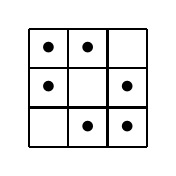
\begin{tikzpicture}[scale=0.5]
\draw[step=1,thick] (0,0) grid (3,3);
\node at (0.5,2.5) {$\bullet$};
\node at (1.5,2.5) {$\bullet$};
\node at (0.5,1.5) {$\bullet$};
\node at (2.5,1.5) {$\bullet$};
\node at (1.5,0.5) {$\bullet$};
\node at (2.5,0.5) {$\bullet$};
\end{tikzpicture}
\end{center}
每行$2$个，每列$2$个，共$6$个。所以最大值是$6$。
\end{solution}

\begin{example}
$10$个球队进行单循环比赛（每两队赛一场），胜得$2$分，平得$1$分，负得$0$分。比赛结束后，总分最多的队至少得了多少分？
\end{example}
\begin{solution}
$10$个队单循环共$C_{10}^2=45$场比赛，每场产生$2$分（胜$2$+负$0$，或平$1$+平$1$），总分$=45\times2=90$分。

如果各队得分尽可能平均，则$90\div10=9$分，平均每队$9$分。但冠军得分至少是$\ge$平均分（由平均值原理），所以冠军至少$9$分。

构造：让所有比赛都平局，则每队$9$分，冠军$9$分。所以冠军至少$9$分。
\end{solution}

\begin{example}
有$n$个城市，需要在它们之间修建道路，使得每两个城市之间都有直达路或经过一个中间城市到达的路（即图的直径为$2$）。最少需要修多少条路？
\end{example}
\begin{solution}
当$n=1$时，$0$条。\\
当$n=2$时，$1$条（直接连）。\\
当$n\ge3$时，最少需要$n-1$条？不，$n-1$条只能形成一棵树，树中两点的距离可能很长。

构造：选一个中心点，与其余$n-1$个点都相连。这样需要$n-1$条路。\\
任意两个非中心点之间：都连接到中心点，距离为$2$。\\
非中心点与中心点之间：直达，距离为$1$。\\
所以$n-1$条路就够了。

能否更少？少于$n-1$条路则图不连通，必定有两点之间没有路径。所以$n-1$是最小值。
\end{solution}

\begin{exercise}
\item $4\times4$的棋盘每行每列最多放$3$个棋子，最多能放多少个？构造一种放法。
\item $8$支球队单循环，胜$2$分、平$1$分、负$0$分，总分最多的队至少得多少分？
\end{exercise}

\sectiontitle{本章小结}

极端原理和组合最值是组合数学中两个高度相关的主题。极端原理的核心是从最特殊的情况入手，利用"最"字推出矛盾；组合最值则要求双向证明——既要构造例子说明能达到多少，又要证明不能再好。两者都是数学竞赛中的常用工具。

\sectiontitle{课后练习}

\subsection*{A组\quad 基础巩固}

\begin{exercise}
\item 在一个$10\times10$的棋盘上放棋子，每行每列最多放$1$个，最多能放多少个？
\item $5$支球队单循环，胜$2$分、平$1$分、负$0$分，总分最多的队至少得几分？
\item $n$个点，任意两点连一条线，最多能画多少条线段？
\end{exercise}

\subsection*{B组\quad 挑战提升}

\begin{exercise}
\item 在一个$8\times8$的棋盘上放棋子，要求任意两个棋子不在同一行也不在同一列，最多能放多少个？有多少种放法？
\item 一个班级有$30$名学生，每个学生至少认识$10$个其他同学。证明：一定存在$3$个学生两两互相认识。
\item 有$n$盏灯排成一圈。每次操作可以选择相邻的$3$盏灯，同时改变它们的状态（亮变灭，灭变亮）。能否通过有限次操作，把所有灯从全灭变成全亮？请分$n$的情况讨论。
\end{exercise}

\vfill
\noindent\rule{\textwidth}{0.4pt}
本章练习答案请参见书末附录。
